\documentclass{article}
\usepackage{geometry}
\special{papersize=60mm,50mm}
\geometry{verbose,paperwidth=60mm,paperheight=50mm,tmargin=2mm,bmargin=2mm,lmargin=2mm,rmargin=2mm}
\usepackage{fontspec}
\usepackage{xunicode}
\usepackage{xltxtra}
\renewcommand{\familydefault}{\sfdefault} 
\usepackage{pgf}
\usepackage[absolute]{textpos}
\usepackage{setspace}

\parindent=0mm

\setlength{\TPHorizModule}{1mm}
\setlength{\TPVertModule}{\TPHorizModule}
\textblockorigin{2mm}{2mm}

\begin{document}

\begin{textblock}{18}[0,0](41,26)
\begin{picture}(1,10)
\put(-10,-45){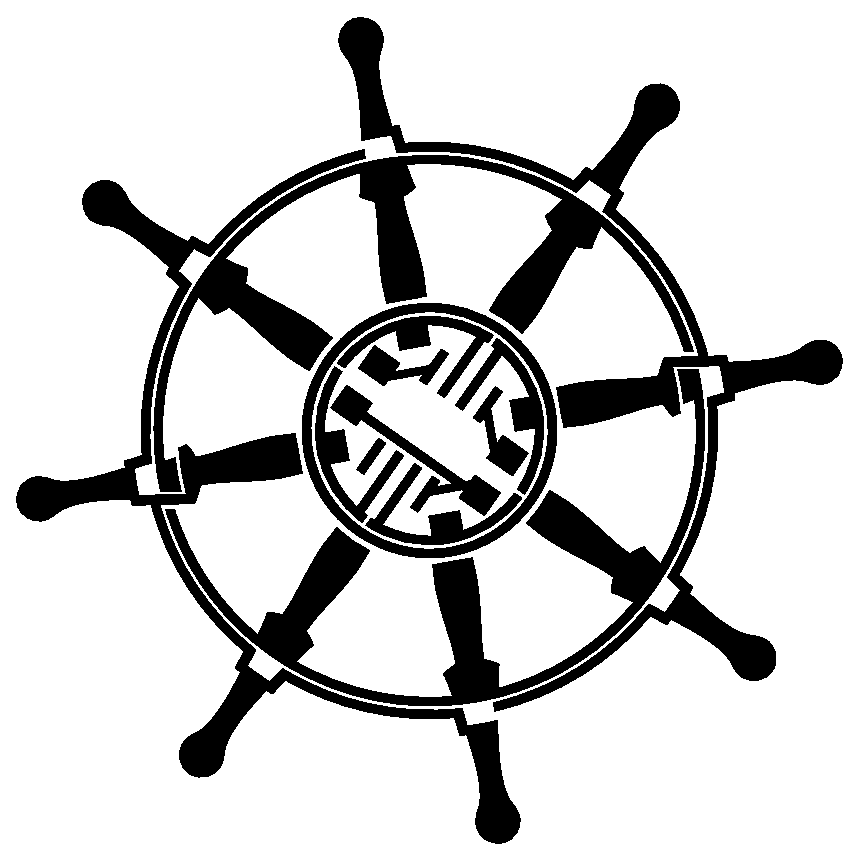
\includegraphics[width=18mm]{techinc.eps}}
\end{picture}
\end{textblock}

\begin{spacing}{.8}
\begin{textblock}{58}[.5,0](28,0)
\begin{center}
\vspace{-3mm}
\textsf{\large \textbf{Congratulations!}} \\
\vspace{1.5mm}
You've caught a travelling book! \\
Enter the BCID below at \textbf{www.bookcrossing.com} to see where it's been, then follow where it goes after you \textbf{READ \& RELEASE} it!
\vspace{1mm}

\end{center}
\end{textblock}
\end{spacing}

\begin{spacing}{.8}
\begin{textblock}{36}[0,1](0,53)
\verb|BCID|
\begin{center}
\vspace{-2mm}
\textsf{\textbf{BCID-HERE}} \vspace{1mm} \\
\end{center}
\vspace{-2mm}
\vspace{6mm}
\end{textblock}
\end{spacing}

\end{document}
